\documentclass{beamer}

\mode<presentation> {
	\usetheme{Berlin}
}

\title[12th International Conference on Large-Scale Scientific Computations, June 10 - 14, 2019, Sozopol, Bulgaria]{
	Solving Combinatorial Puzzles with Parallel Evolutionary Algorithms
}

\author{Todor Balabanov, Stoyan Ivanov, Rumen Ketipov}

\date{10-14.VI.2019}

\institute[IICT-BAS, LSSC'19] {
	Institute of Information and Communication Technologies \\ 
	Bulgarian Academy of Sciences \\
	\medskip
	\textit{todorb@iinf.bas.bg}
}

\begin{document}

\begin{frame}
\titlepage
\end{frame}

\begin{frame}
\frametitle{Overview}
\tableofcontents
\end{frame}

\section{Introduction}

\begin{frame}
\center \huge{Introduction}
\end{frame}

%\begin{frame}
%\frametitle{Clustering}
%\begin{itemize}
%  \item Separation of the data set in set of groups
%  \item Straight clustering - each data sample belongs exactly to only one group
%  \item Fuzzy clustering - each data sample has varying degree of membership to different groups
%\end{itemize}
%Optimal clustering is data set separation which minimizes the distance inside the cluster and maximizes the distance between the clusters
%\end{frame}
%
%\begin{frame}
%\frametitle{Self-Organizing Maps}
%\begin{itemize}
%  \item Proposed by Teuvo Kohonen in the 1980s
%  \item Have application in meteorology, oceanography, project prioritization and selection, seismic facies analysis for oil and gas exploration, failure mode and effects analysis, creation of artwork and many other areas
%  \item They are very useful for visualization by data dimensions reduction
%\end{itemize}
%\end{frame}
%
%\begin{frame}
%\frametitle{SOM in General}
%\begin{itemize}
%  \item Unsupervised competitive learning is used
%  \item Classify input data in predefined number of clusters
%  \item When the net has fewer nodes it achieve results similar to K-means clustering
%\end{itemize}
%\end{frame}
%
%\section{Neighborhood Function Proposition}
%
%\begin{frame}
%\center \huge{Neighborhood Function Proposition}
%\end{frame}
%
%\begin{frame}
%\frametitle{SOM Training}
%\begin{itemize}
%  \item The network consists of a grid with units
%  \item The units are connected to adjacent units with a neighborhood relation
%  \item The network forms an elastic mesh
%  \item Data samples lying near each other in the input space are mapped into nearby grid units
%\end{itemize}
%\end{frame}
%
%\begin{frame}
%\frametitle{Neighborhood Function}
%\begin{itemize}
%  \item It gives scaling factor for the distance between one neuron and other neurons in each step
%  \item The simplest form of a neighborhood function gives 1 for the closest nodes and 0 for all other
%  \item The most used neighborhood function is a Gaussian function
%\end{itemize}
%\end{frame}
%
%\begin{frame}
%\frametitle{Fading Cosine}
%\begin{figure}[h]
%  \centering
%  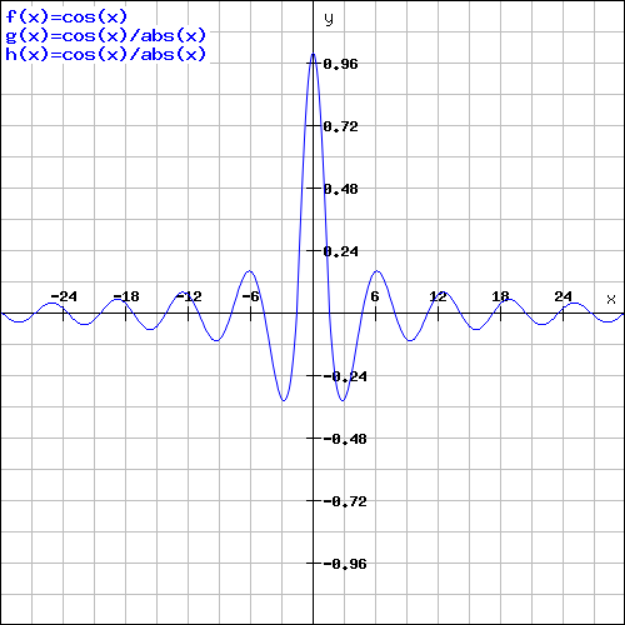
\includegraphics[width=0.45\linewidth]{fig01a}
%\label{fig01a}
%\end{figure}
%\begin{equation} \label{equ01}
%f(x) = 
%	\begin{cases} 
%		cos(x) & -\pi/2 < x < \pi/2 \\
%		\frac{cos(x)}{|x|} & +\pi/2 \geq x \leq -\pi/2 \\
%	\end{cases}
%\end{equation}
%\end{frame}
%
%\begin{frame}
%\frametitle{Exponential Regulated Cosine}
%\begin{figure}[h]
%  \centering
%  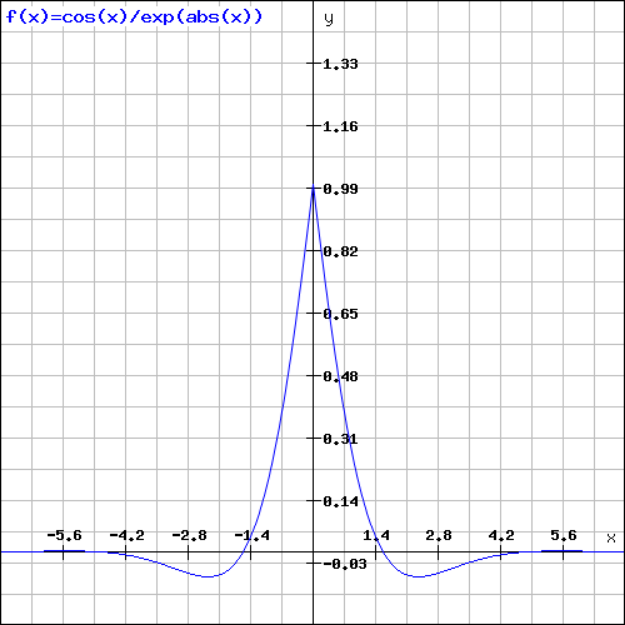
\includegraphics[width=0.45\linewidth]{fig01b}
%\label{fig01b}
%\end{figure}
%\begin{equation} \label{equ02}
%f(x) = \frac{cos(x)}{e^{|x|}}
%\end{equation}
%\end{frame}
%
%\section{Experiments and Results}
%
%\begin{frame}
%\center \huge{Experiments and Results}
%\end{frame}
%
%\begin{frame}
%\frametitle{Experimental Setup}
%\begin{itemize}
%  \item All experiments are done in C as a programming language
%  \item Single processor desktop machine - Intel Core i5, 2.3 GHz, 2 Cores, 8GB RAM and Mac OS X 10.13.6, Apple LLVM version 9.1.0
%  \item The source code is available at: 
%  http://github.com/Coding-Sunday-Sofia/Kohonen
%\end{itemize}
%\end{frame}
%
%\begin{frame}
%\frametitle{Experimental Data}
%\begin{figure}[h]
%  \centering
%  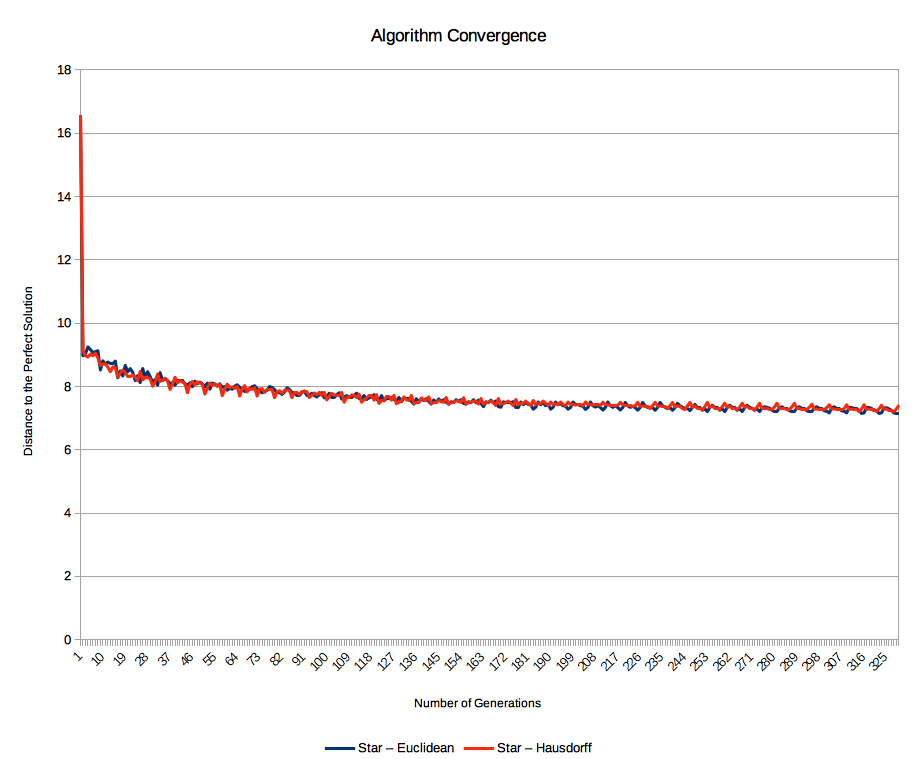
\includegraphics[width=0.9\textwidth]{fig03}
%  \label{fig03}
%\end{figure}
%Rents and living area data set
%\end{frame}
%
%\begin{frame}
%\frametitle{Gausssian Test}
%\begin{figure}[h]
%  \centering
%  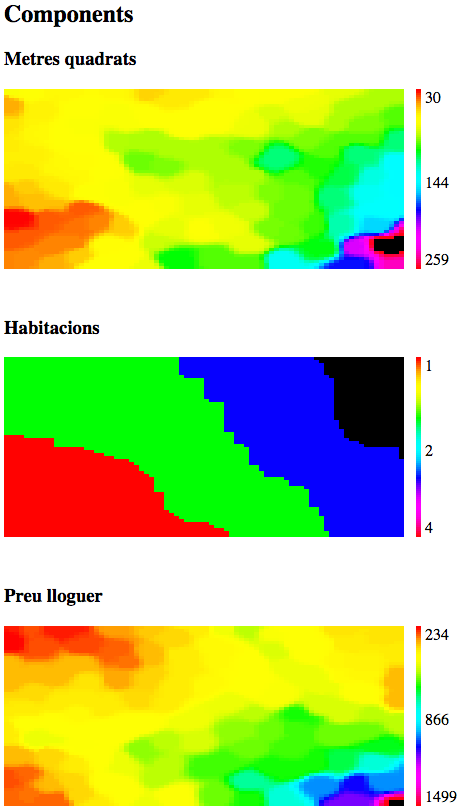
\includegraphics[width=1.0\textwidth,height=0.6\textwidth]{fig02a}
%  \label{fig02a}
%\end{figure}
%\end{frame}
%
%\begin{frame}
%\frametitle{Fading Cosine Test}
%\begin{figure}[h]
%  \centering
%  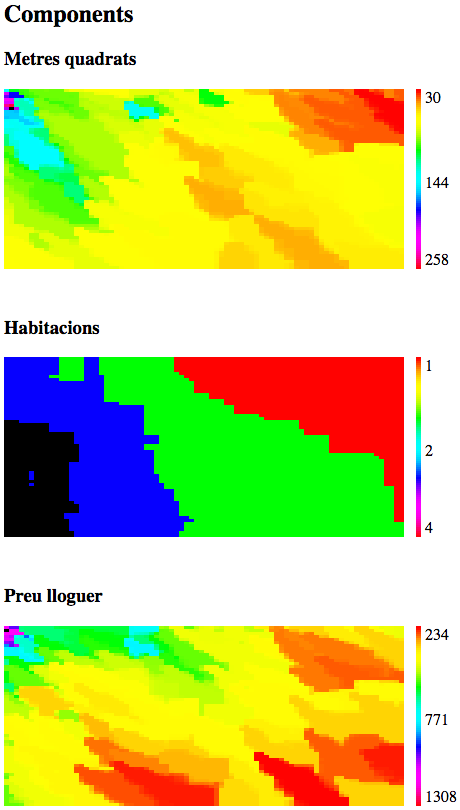
\includegraphics[width=1.0\textwidth,height=0.6\textwidth]{fig02b}
%  \label{fig02b}
%\end{figure}
%\end{frame}
%
%\begin{frame}
%\frametitle{Exponential Regulated Cosine Test}
%\begin{figure}[h]
%  \centering
%  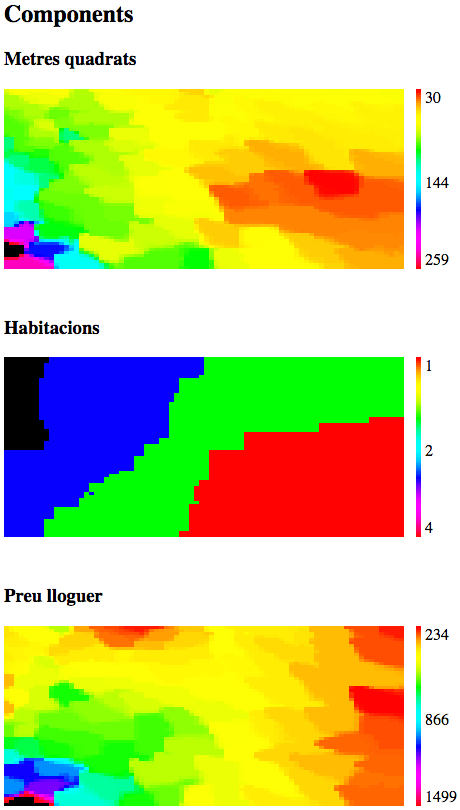
\includegraphics[width=1.0\textwidth,height=0.6\textwidth]{fig02c}
%  \label{fig02c}
%\end{figure}
%\end{frame}

\section{Conclusions}

\begin{frame}
\center \huge{Conclusions}
\end{frame}

\begin{frame}
\frametitle{Concluding Remarks}
\begin{itemize}
  \item Addition of Hausdorff distance component improves the performance of the genetic algorithm
  \item Calculation of the Hausdorff distance is a little bit slower than the calculation of the Euclidean distance
  \item Better solution fitness estimation generally leads to genetic algorithm convergence improvement
\end{itemize}
\end{frame}

\begin{frame}
\frametitle{Questions and Answers}
\center \huge{Thank you for the attention!}
\end{frame}

\end{document}
